%https://github.com/edasubert/beamerMaterialDesign


\documentclass{beamer}
\usefonttheme{professionalfonts}
\usepackage{fontspec}
\usepackage{mathtools}
\usepackage{unicode-math}
\usepackage{pgfpages}
\usepackage{comment}
\usepackage{listings}
\usepackage[polish]{babel}

% \setbeameroption{show notes on second screen}

\title{Ostatecznie spójne transakcje}
\date{18 maja 2018}
\author{Jan Bajer\\Adam Pioterek}

\usetheme{material}

\useLightTheme{}
\usePrimaryIndigo{}
\useAccent{4caf50}{087f23}

\lstdefinelanguage{js}{
    keywords={const, typeof, new, true, false, catch, function, return, null, catch, switch, var, if, in, while, do, else, case, break, global, match, yield, with, array, print, foreach, not, entries, flush},
  keywordstyle=\color{blue}\bfseries,
  keywords=[2]{bool, string, cint, int, cstring, object},
  keywordstyle=[2]\color{orange}\bfseries,
  identifierstyle=\color{black},
  sensitive=false,
  comment=[l]{//},
  morecomment=[s]{/*}{*/},
  commentstyle=\color{purple}\ttfamily,
  stringstyle=\color{red}\ttfamily,
  morestring=[b]',
  morestring=[b]"
}
\lstset{
   language=js,
   extendedchars=true,
   basicstyle=\tiny\ttfamily,
   showstringspaces=false,
   showspaces=false,
   tabsize=2,
   breaklines=true,
   showtabs=false,
   numbers=left
}


\begin{document}

\begin{frame}
\titlepage{}
\end{frame}

\begin{frame}{Źródło}
    \begin{card}
        Na podstawie:
        \begin{itemize}
            \item Burckhardt et.\ al. “Eventually Consistent Transactions”
            \item Burckhardt et.\ al. “Cloud Types for Eventual Consistency”
        \end{itemize}
    \end{card}
\end{frame}

\section{Jan}

\begin{frame}{Opis problemów wg wstępu z Cloud Types}
\end{frame}

\begin{frame}{Definicje Sequential, Eventual, Revision Consistency}
\end{frame}

\begin{frame}{Revision Graphs, porównanie rewizji i transakcji}
\end{frame}

\begin{frame}{Historie?}
\end{frame}

\section{Adam}

\begin{frame}[fragile]{Typy chmurowe}
    \begin{card}
        \begin{itemize}[<+->]
            \item automatycznie współdzielone,
            \item przewidywalność podczas współbieżnych modyfikacji,
            \item automatyczne rozwiązywanie konfliktów,
            \item używają \textit{revision consistency}
        \end{itemize}
    \end{card}
    \only<5> {
        \begin{card}[Informatyczny humor]
            globalne zmienne, \textit{dosłownie}
        \end{card}
    }
    % We believe that the essential features of our system can be incorporated in most real-world static or dynamic languages in a seamless way. We currently have a partial implementation directly in the TouchDevelop language and as a library in C#.
    % Conceptually, the cloud stores the main revision, while devices maintain local revisions that are periodically synchronized
\end{frame}

\begin{frame}[fragile]{Lista zakupów}
    \begin{card}
        \begin{lstlisting}
global totalItems: CInt;
array Grocery[name: String] {
    toBuy: CInt;
}

function ToBuy(name: String, count: Int) {
    totalItems.add(count);
    Grocery[name].toBuy.add(count);
}

function Bought(name: String, count: Int) {
    totalItems.add(-count);
    Grocery[name].toBuy.add(-count);
}

function Display() {
    foreach g in entries Grocery.toBuy {
        Print(g.toBuy.get() + " " + g.name);
    }
    Print(totalItems.get() + " total");
}
        \end{lstlisting}
    \end{card}
\end{frame}

\begin{frame}[fragile]{Lista zakupów (cd.)}
    \begin{card}
        \begin{lstlisting}
function main() {
    bool done = false;
    while (not done) {
        yield();  // allow send/receive of updates
        match (NextUserCommand()) with {
            buy s n:
                ToBuy(s, n);
            bought s n:
                Bought(s, n);
            display:
                Display();
            quit:
                done = true;
        }
    }
}
        \end{lstlisting}
    \end{card}
    % Co się tu dzieje
\end{frame}

\begin{frame}{\texttt{yield}}
    % The important part is the yield statement. Essentially, the yield statement gives the runtime system the permission to both (1) propagate changes made locally to the replica to other devices, and (2) apply changes made by other devices to the local replica. yield is nonblocking and guaranteed to execute very quickly. yield does not force synchronization: it is perfectly acceptable for yield to do nothing at all (which is in fact all it can do in situations where the device is not connected). Another way to describe the effect of yield is that the absence of a yield guarantees isolation and atomicity; yield statements thus partition the execution into a form of transaction (called eventually consistent transactions in [1]). Effectively, this implies that everything is always executing inside a transaction.
    \begin{card}
        \begin{itemize}[<+->]
            \item pozwala na synchronizację,
            \item ale jest nieblokujący (nie wymusza --- może nie robić nic)
        \end{itemize}
    \end{card}
    \onslide<3->{
        \begin{card}
            \begin{description}[<+->]
                \item[A] jeśli nie czekamy na odpowiedź od serwera, wysyłamy aktualną rewizję do serwera po forku nowej rewizji,
                \item[B] jeśli nadeszła (przed \texttt{yield}) rewizja od serwera, łączymy do niej rewizję lokalną,
                \item[C] jeśli oczekujemy odpowiedzi, ale jeszcze nie przyszła, nie robimy nic.
            \end{description}
        \end{card}
    }
\end{frame}

\begin{frame}{\texttt{yield} --- przykład}
    \only<1> {
        \begin{card}
            \begin{figure}[ht]
                \centering
                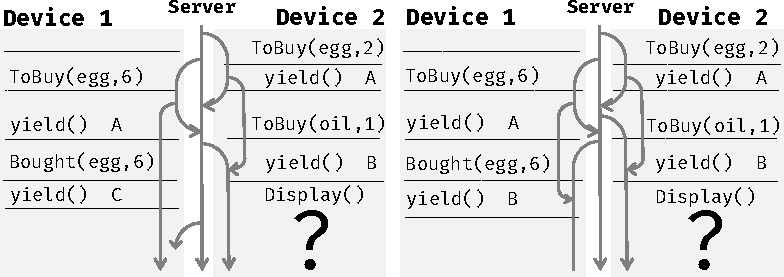
\includegraphics[width=\textwidth]{yieldABC_question.pdf}
            \end{figure}
        \end{card}
    }
    \only<2> {
        \begin{card}
            \begin{figure}[ht]
                \centering
                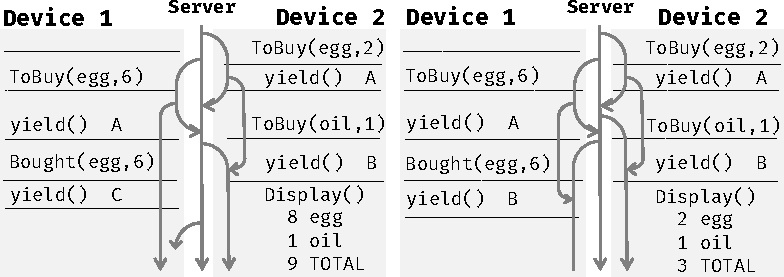
\includegraphics[width=\textwidth]{yieldABC_answer.pdf}
            \end{figure}
        \end{card}
    }
    % Program execution is nondeterministic if multiple devices are involved. Both of the following revision diagrams represent possible executions of the grocery list example. Because of timing differences, the Display() on device 2 may either see the first update by device 1 (left) or not see it (right).
    % As long as clients repeatedly call yield, and as long as messages are eventually delivered (using retransmission if necessary), eventual consistency is achieved.
    % Zadanko
\end{frame}

\begin{frame}[fragile]{Silniejsza spójność}
    \begin{card}
        Czasami potrzebna silniejsza spójność (zamawianie biletów, wypłata pieniędzy).
    \end{card}
    \begin{card}[Cóż może pójść nie tak?]
        \begin{lstlisting}
array Seat [row: Int, letter: String] {
    assignedTo: CString;
}

function NaiveReserve(seat: Seat, customer: String) {
    if (seat.assignedTo.get() == "")
        seat.assignedTo.set(customer);
    else
        Print("reservation failed");
}
        \end{lstlisting}
    \end{card}
    % Unfortunately, this does not work as desired: a seat may appear empty in the local revision, but already be filled on the server. In this case, the NaiveReserve function would appear to succeed, but in fact may overwrite another reservation once the update reaches the server.
\end{frame}

\begin{frame}[fragile]{Silniejsza spójność --- podejście \#2}
    % We fix this problem by introducing a primitive operation setIfEmpty for the cloud type CString. This operation sets the string only if it is currently empty, and this condition is reevaluated when the update operation is applied on the server. Thus, existing reservations are never overwritten.
    \begin{card}
        Wprowadźmy operację \texttt{CString.setIfEmpty(String)}.
    \end{card}
    \begin{card}[Lepiej?]
        \begin{lstlisting}
array Seat [row: Int, letter: String] {
    assignedTo: CString;
}

function NaiveReserve(seat: Seat, customer: String) {
    seat.assignedTo.setIfEmpty(customer);
    yield();
    if (seat.assignedTo.get() != customer)
        Print("reservation failed");
}
        \end{lstlisting}
    \end{card}
\end{frame}

\begin{frame}[fragile]{Silniejsza spójność --- podejście \#3}
    % However, yield is still not sufficient to force mutual exclusion, since we cannot tell when the update has reached the server. Thus we support an additional synchronization primitive called flush. Upon flush, execution blocks until (1) all local updates have been applied to the main revision, and (2) the result has become visible to the local revision.
    \begin{card}
        Wprowadźmy \texttt{flush}.
    \end{card}
    \begin{card}[Obiecuję --- to już jest koniec.]
        \begin{lstlisting}
array Seat [row: Int, letter: String] {
    assignedTo: CString;
}

function NaiveReserve(seat: Seat, customer: String) {
    seat.assignedTo.setIfEmpty(customer);
    flush;
    if (seat.assignedTo.get() != customer)
        Print("reservation failed");
}
        \end{lstlisting}
    \end{card}
    % Since flush could block indefinitely if the device is not connected, our implementation supports the specification of a timeout.
\end{frame}

\begin{frame}[fragile]{Silniejsza spójność --- Podsumowanie}
    \begin{card}[No dobrze --- tylko po co?]
        \begin{itemize}[<+->]
            \item ten model jest równie kosztowny jak pamięć współdzielona i zamki,
            \item ten przykład nie reprezentuje aplikacji, do których ten model się nadaje,
            \item wręcz przeciwnie --- do aplikacji wymagających częstych i silnych synchronizacji bardziej nadaje się tradycyjne podejście do transakcji.
        \end{itemize}
    \end{card}
\end{frame}

\begin{comment}

\section{Intro}

\begin{frame}{Overlay}
    \begin{card}
        \begin{itemize}[<+->]
            \item hello
            \item there
        \end{itemize}
    \end{card}
    \note{This shows overlay}
\end{frame}

\begin{frame}{Card}
    \begin{card}
        {\color{accent} \textbackslash{}begin\{card\}\\[2mm]}
        \null\qquad \textit{[your content here]}\\[2mm]
        {\color{accent} \textbackslash{}end\{card\}}
    \end{card}
\end{frame}

\section{Unicode}

\begin{frame}{TitleCard}
    \begin{card}[Some unicode in formulas:]
        \begin{equation}
            α² + β² = γ²
        \end{equation}
        And a fraction: ½.
    \end{card}
    \note{Wow! Unicode works}
\end{frame}

\end{comment}

\end{document}
